\chapter{Design}

The design of Snapstore had two steps. The first was to identify the purposes of a VCS. The second was to create a conceptual model composed of concepts that fulfilled the purposes of a VCS.

\section{Purposes of Version Control}

The six purposes of a VCS identified in \cite{RossoJackson} were used in the design of Snapstore. A purpose graph is included in Figure 3-1, where each subpurpose points to its parent purpose. The purposes are classified into five categories: data management, change management, collaboration, parallel development, and disconnected development.

\begin{figure}

\includegraphics[max width= \linewidth]{PurposeGraph}
\caption{Purpose Graph of Version Control Systems.}
\label{arm:fig1}
\end{figure}

\textbf{Data Management} deals with the notion of backup. In case of failure, this data needs to be stored persistently and be able to be retrieved. This purpose addresses risks associated with development such as accidental deletion and incorrect saves, not just machine failure. The ability to track and untrack files gives user control over what files will be persistently stored.

The second class, \textbf{change management}, deals with managing these edits. Grouping changes allows the user to divide the history of a file or files in logical segments. Groups like current file state help users accurately model the state of their project. Tagging these groups as coherent points in development aid in administrative and managerial tasks associated with long or large projects. These coherent points in the project can then be returned to by reverting the project to reflect the versions of files in that collection.

\textbf{Collaboration} concerns a system shared by multiple users. Synchronizing the changes of collaborators on that system allows their edits to be amalgamated in such a way that conflicts are avoided when possible and made explicit when they cannot be avoided.

\textbf{Parallel Development}, the fourth class, mainly deals with supporting parallel lines of development. Switching between parallel lines, as well as merging parallel lines are needed to fully support parallel development. This purpose allows users more flexibility to isolate parts of their work from others, and to develop without affecting the main line.

The final class, \textbf{Disconnected Development}, allows operations to be performed in a disconnected mode. This motivates any work that a user can do in an offline setting or in a setting where a user is willingly disconnected from their collaborators.

\section{Conceptual Model}

Once the purposes of VCSs were defined, a conceptual model that addressed those purposes and that was aligned with conceptual design theory \cite{Jackson} was created. A mapping of each Snapstore concept to its motivating purpose is shown in Table 3.1. Table 3.2 shows each Snapstore concept and its operational principle. A graphical representation of the conceptual model, using the notation for extended entity-relationship diagrams as used in \cite{Jackson}, is shown in Figure 3-2.

\begin{table}
\begin{tabular}{ |p{5cm}||p{9cm}|}
 \hline
 \textbf{Concept} & \textbf{Motivating Purpose}\\[8pt]
 \hline
 Snapshot & Make a set of changes to a file persistent\\[8pt]
 %
 Create, Update, Rename, and Delete Snapshot & Track various types of changes to a file\\[8pt]
 %
 Snapstore Folder & Provide a platform for users to edit files\\[8pt]
 %
 Tracked File & Mark files whose changes should be saved\\[8pt]
 %
 Untracked File & Mark files whose changes should be ignored\\[8pt]
 \hline
 Group & Group logically related changes together\\[8pt]
 Head Snapshot & Easy way of naming the current snapshot\\[8pt]
 Tag & Represent and record coherent points in history\\[8pt]
 \hline
 Upstream Repository & Synchronize changes of collaborators\\[8pt]
 \hline
 Branch & Support parallel lines of work\\[8pt]
 Conflict Snapshot & Mark snapshots with unresolved conflicts\\[8pt]
 Merge Snapshot & Indicate that a snapshot is the result of a merge\\[8pt]
 \hline
 Local Repository & Do work in disconnected mode\\[8pt]
 \hline
\end{tabular}
\caption{Concepts of Snapstore and their motivating purposes.}
\end{table}

\begin{table}
\begin{tabular}{ |p{5cm}||p{11cm}|}
 \hline
 \textbf{Concept} & \textbf{Operational Principle}\\[8pt]
 \hline
 Snapshot & Whenever a file is saved to disk, a snapshot containing that file's contents is created\\[8pt]
 %
 Create, Update, Rename, and Delete Snapshot & Whenever a specific type of action on a file results in a disk save, the same type of snapshot is created\\[8pt]
 %
 Snapstore Folder & If a user edits any tracked files within the Snapstore folder, Snapstore will create a snapshot for that file\\[8pt]
 %
 Tracked File & When a user tracks a file within the Snapstore folder, snapshots will be created for that file\\[8pt]
 %
 Untracked File & When a user untracks a file within the Snapstore folder, no snapshots will be created for that file\\[8pt]
 \hline
 Group & When a user places a set of snapshots in a group, they can be found later with the group's name\\[8pt]
 Head Snapshot & Whenever a user inspects a file, the contents of that file correspond to the contents of its head snapshot\\[8pt]
 Tag & When a user places a tag on a group, that group can be found using the tag's name, and every file within that group can be reverted to it's associated snapshot content within that group at the same time\\[8pt]
 \hline
 Upstream Repository & Whenever a user makes a change on a branch that more than user has access to, that change is propagated by the upstream to all other collaborators on that branch\\[8pt]
 \hline
 Branch & When the user switches branches, Snapstore hides the old branch's data, shows them the current branch's data, and allows them to start adding data to the current branch\\[8pt]
 Conflict Snapshot & If there is a conflict when merging two head snapshots, the result is a conflict snapshot, which shows where the conflict is\\[8pt]
 Merge Snapshot & If there is no conflict when merging two head snapshots, the result is a merge snapshot\\[8pt]
 \hline
 Local Repository & Whenever the user is offline, any changes to Snapstore are saved persistently in the local repository\\[8pt]
 \hline
\end{tabular}
\caption{Concepts of Snapstore and their operational principles.}
\end{table}

\begin{figure}
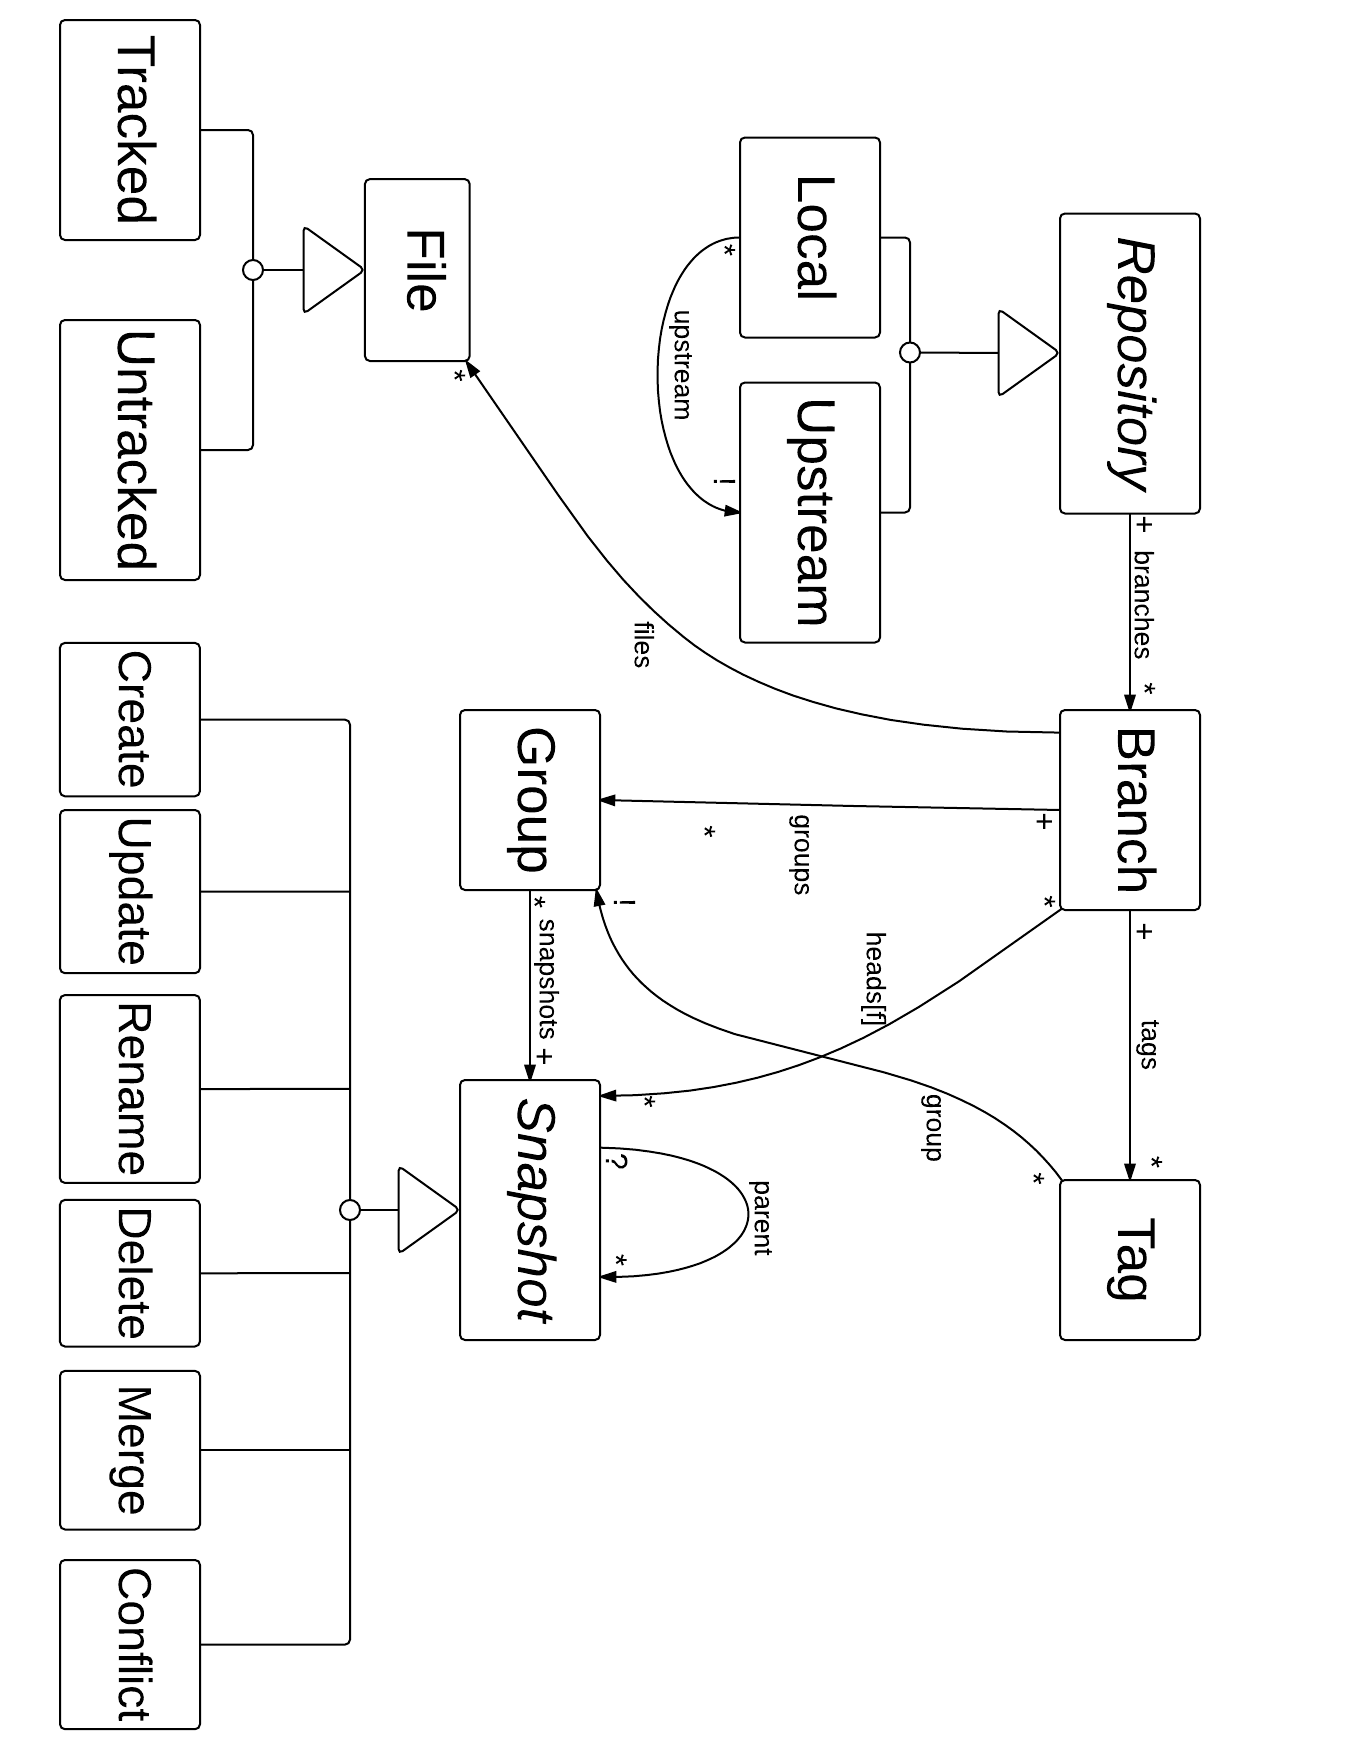
\includegraphics[max width= \linewidth]{ConceptModel}
\caption{Concept Model of Snapstore.}
\label{arm:fig1}
\end{figure}

\subsection{Data Storage --- Snapshot}

Persistent data storage in Snapstore is achieved with the notion of a \textit{snapshot}. A snapshot is a saved state of a file. Snapshots record updates, renames, moves, deletes, along with merges and conflicts. The \textit{head} snapshot for any given file is the most recent snapshot made for that file and reflects the current content of that file on that machine. 

This type of snapshot dictates the values of that snapshot's attributes. Create snapshots have no parent. Update snapshots have a parent, a child, and content. Rename snapshots have a different filename than their parent. Delete snapshots have no content, though they still have a parent and can therefore be placed in the snapshot graph. Merge snapshots have more than one parent, and conflict snapshots are merge snapshots that have conflict markers in their data.

All snapshots have parent snapshots and child snapshots. The snapshots of a file are related by the graph they create with these parent/child relationships. This ordering forms the snapshot graph described in section 2.1.1. Each unique (branch, file) tuple is represented by its own snapshot graph. A snapshot can have multiple parents if it is the result of a merge operation. 

The snapshot graph is guaranteed to be an in-order description of snapshots a specific client has made to a file in a branch. There is no operation on the client that distorts the ordering of snapshots in the graph. The only operation that can alter the graph occurs when another client's snapshot is inserted in the graph. However, even if snapshots are inserted into a user's snapshot graph, the user's ordering of locally made snapshots stays intact.

Any file, identified by its snapshot graph, can either be tracked or untracked. Edits made to untracked files will not create snapshots.

\subsection{Grouping Changes --- Group}

A \textit{group} is an assembly of related snapshots. A group must contain at least one snapshot, but there are no restrictions on what kinds of snapshots can be in the group or what their relationship must be. The same snapshot can exist in more than one group. It is up to the user to decide what makes a group of snapshots logically related. This allows flexibility in projects and development strategy.

Groups are an attribute of a specific branch. Even if two group contain the same snapshots across different branches, those groups are different because they exist on different lines of development. Any group can be given a name for identification for the user.

\subsection{Recording Coherent Points --- Tag}

The notion of a \textit{tag} allows users to label logical milestones in their work. They describe groups but have an added function over a group's name: they describe the status of the group as representing a coherent point. Here, coherent means that the project is in a state that is ready for further development or work, though the definition will differ from team to team \cite{RossoJackson}. 

Tags will always describe groups that are perfectly vertical. That is, at most one snapshot from any file is in the group. An example of this is tagging every head snapshot in a branch at a given time with the tag ``Submitted to Scientific Journal'' or ``Version 1.0''.

Tags are also an attribute of the branch. This means that they must be created inside a of an independent line of development. They can be copied across branches when merging and cloning, but they stay a fundamental attribute of the branch concept.

\subsection{Support Parallel Lines --- Branch}

In Snapstore, the concept of a \textit{branch} supports parallel and independent lines of development. These branches are completely separate from each other. They facilitate the appropriate partitioning of data.

The branch houses three of the other main concepts in Snapstore: snapshots, groups, and tags. All three of those concepts exist within the confines of a branch. All of these things together consitute a line of development, and so the branch is the conceptual representation of that line.

Branches make up a repository, whether that repository is local or upstream. Switching between them constitutes changing the line of development, project, folder, or anything that delineates the user's work. Switching between two branches on a single local repository that are stored on different upstreams has no averse effects due to their independence.

Branches can also be shared between multiple users. User on a shared branch can work independently, confident that any changes they make will not be lost. These changes, whether they deal with snapshots, groups, or tags, are be persistent. New changes can come in through the network while a user is working, but it won't affect their ability to send their own changes.

Branches can be merged together, synchronizing the parallel development. This simply involves combining each branch's individual snapshot, group, and tag data together as explained in chapter 2.2.3.

\subsection{Synchronize Changes of Collaborators --- Upstream Repository}

Snapstore uses a centralized data storage system that holds all connected branch data, called an \textit{upstream repository}, or upstream for short. While users do not necessarily have to use an upstream for their local repository, it is the only way to collaborate with other users on any branch in that local repository.

Every local repository can have one upstream, and it does not have to be the default Snapstore upstream. This allows the user to choose the location through which their data passes.

All changes that occur at the branch level (branches, snapshots, groups, tags) are reflected in any connected upstream. There, the upstream can see if any other users have access to that branch and it can push the changes down to them.

\subsection{Disconnected Work --- Local Repository}

The ability to leverage the benefits of a VCS without needing an internet or network connection is handled by the \textit{local repository}. The local repository affords all of the same relationships to other concepts as the upstream. That is, it is a collection of branches, which are in turn collections of snapshots, groups, and tags.

The local repository can have one or zero upstreams attached to it. It is through these upstreams that shared data will propagate to collaborators.

\subsection{Discussion}

During the design process, there were many decisions made that had lasting tradeoffs for Snapstore. The main tradeoffs are explored below.

\subsubsection{Granularity of a Snapshot}

The decision of what a snapshot would represent was the first design decision we encountered. Either a snapshot could represent the state of a file, or it could represent the state of every file in a branch. 

The first reason we decided to make the snapshot describe the state of a single file was that it was more intuitive to a typical user. If a user was to save a file and create a snapshot, they would expect that snapshot to relate to the object they just interacted with, that file. They would not expect it to relate to every file in the branch.

Another reason for this decision was the necessity of the group concept. In many VCSs such as Git and Mercurial, saving changes couples together the act of saving changes with the act of grouping changes, resulting in an overloaded concept \cite{Jackson}. We separated the saving of changes with grouping those changes; the snapshot represents the state of a single file, instead of a group of files.

One downside of this approach is the additional computation needed to compute the current state of a branch. In Git, the current state is the head commit. In Snapstore, we need to calculate this by grabbing all of the head snapshots for a branch. This is typically trivial, so the tradeoff is beneficial.

\subsubsection{The Upstream}

Different VCSs and file sharing systems have their own ways of handling storage. Git, for example, use a decentralized storage system. Dropbox and SVN, on the other hand, use a centralized system. When deciding which model to use for our upstream, we looked at both models' pros and cons. Centralized VCSs are easier to learn and use \cite{Brindescu}, but they require an Internet connection and don't allow users to share directly with each other. Distributed VCSs do allow users to work offline and share with each other, but they also have more space requirements because the version history for every file exists on every machine.

Snapstore uses a hybrid centralized/decentralized upstream model. On the surface, it is centralized because all collaboration must take place via the upstream repository. That is, any data a user wants to collaborate on with another user must first go through a centralized repository.

But, Snapstore is also decentralized because users have a local repository, where actions can be made without requiring an active connection to the upstream. Snapstore users each have all of their data on their own machine, just like in a decentralized VCS. Because of this, users can work offline, without checking out a central repository.

There are downsides to this hybrid model. Because Snapstore local repositories can only have one upstream, shared data will always be controlled by a single, centralized entity. Because there is no push/pull model in Snapstore, this machine must always be online in order to facilitate collaboration. Users also cannot share directly with a subset of collaborators on a shared branch. They can, however, work around this limitation by creating new branches with new sets of users.

This hybrid model a balance between the simplicity of a centralized model and some of the power of a decentralized system. The centralized model is easier for the majority of users to use, and it has a faster learning curve \cite{Brindescu}. In Snapstore, the data on the upstream is indeed ``blessed'', and so it is centralized. However, by offering a local repository alongisde and potentially independent from the upstream, Snapstore has some characteristics of a decentralized system.

\subsubsection{File Names}

Whether or not to make the file name a property of a file or the identifier for a file was an important decision for Snapstore. Systems like Git use the file name as an identifier for a file. Because of this decision, renames to a file are sometimes processed as deleting that file and creating a new file, causing much consernation among users, especially novices \cite{RossoJackson}.

We wanted to be able to fully support renaming files in Snapstore, so file names in Snapstore are simply a property of the file. Each snapshot in a given snapshot graph will have the same file id. When branch merging occurs, only snapshot graphs with the same file id will be merged. The merge operation will look back over a file's two snapshot graphs for a common ancestor and perform a standard three-way merge. This allows Snapstore to accurately handle renames and merges.



